\begin{frame}{Iptables}

	\center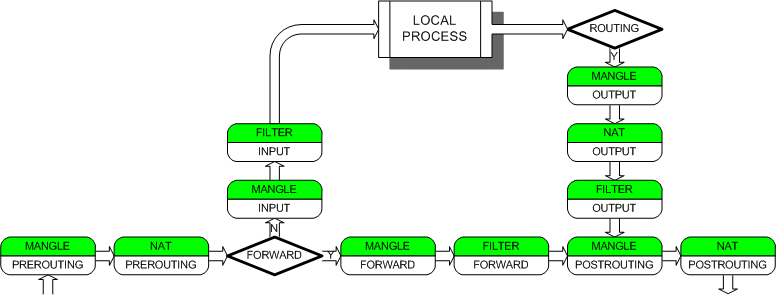
\includegraphics[width=1\textwidth]{../../slides/networking/06-iptables.png}

\end{frame}

\begin{frame}{Iptables}

	\center{\bf iptables -t <table> -L}
	\center{\bf iptables -t <table> -F}
	\bigskip

	\begin{itemize}
	\begin{columns}
		\column{0.3\textwidth}

			\item filter -- файерволл
				\begin{itemize}
					\item INPUT
					\item FORWARD
					\item OUTPUT
				\end{itemize}
		\column{0.3\textwidth}
			\item nat -- преобразования адресов
				\begin{itemize}
					\item PREROUTING
					\item INPUT
					\item OUTPUT
					\item POSTROUTING
				\end{itemize}
		\column{0.3\textwidth}
			\item mangle -- специальные  изменения  пакетов (TOS, TTL, MARK)
				\begin{itemize}
					\item PREROUTING
					\item INPUT
					\item FORWARD
					\item OUTPUT
					\item POSTROUTING
				\end{itemize}
		\end{columns}
	\end{itemize}

\end{frame}


\begin{frame}{Iptables: примеры}

	\center{\bf iptables -t <table> <CRITERIA> <TARGET>}
	\small
	\begin{itemize}
		\item filter:\\
			{\tt iptables -A INPUT -s 192.168.0.1/24 -p UDP -j REJECT -{}-reject-with icmp-host-unreachable}\\
			{\tt iptables -A INPUT -d 192.168.0.1/24 -p TCP -j DROP}
		\item nat:\\
			{\tt iptables -A POSTROUTING -t nat -s 192.168.1.0/24 -j MASQUERADE}\\
			{\tt iptables -t nat -A PREROUTING -p tcp -d 192.168.251.1 
			--dport 8080 -{}-sport 1024:65535 -j DNAT -{}-to 192.168.1.200:8080}
		\item mangle:\\
			{\tt iptables -A PREROUTING -t mangle -p tcp -{}-dport 22 -j MARK -{}-set-mark 100}\\
			{\tt ip route add default dev eth0 table 1}\\
			{\tt ip rule add fwmark 100 table 1}
	\end{itemize}

\end{frame}


\begin{frame}[fragile]{Упражнение}
    \begin{block}{Внутренняя сеть: маскарадинг}
        \begin{enumerate}
            \item Добавить в netns 'A' правило для таблицы {\tt nat},
                включающее маскарадинг для IP-адреса, использующегося в netns 'B'
            \item Запустить {\tt ping -n <IP>} в netns 'B'\\
                IP -- адрес соседа для {\tt ethA0}
            \item Запустить {\tt tcpdump -i ethA0 icmp} в netns 'A'
            \item Запустить {\tt tcpdump -i eth0 icmp} на хосте (без использования netns)
            \item Запретить входящий ''{\tt ping}'' для {\tt ethA0}:\\
                {\tt iptables -A INPUT -i ethA0 -p icmp -j REJECT --reject-with icmp-host-unreachable}
        \end{enumerate}
    \end{block}
\end{frame}
